\documentclass[11pt,a4paper]{ctexart}
\usepackage{siunitx} % 用于处理单位
\usepackage{amsmath} % 用于数学公式
\usepackage{graphicx} % 用于插入图片
\usepackage{array} % 用于表格的多行多列
\usepackage{multirow} % 用于表格的多行合并
\usepackage[margin=1in]{geometry} % 设置页面边距
\usepackage{booktabs} % 更美观的横线
\usepackage{caption}  % 用于调整标题样式
\usepackage{placeins}
\usepackage{titlesec} % 用于自定义标题格式
\usepackage{dcolumn}
\usepackage{amssymb}
\usepackage{bm}
\usepackage{hyperref}       % 建议最后加载 hyperref
\usepackage{multimedia}     % 提供 \movie 和 \sound 命令
\usepackage{media9}
\usepackage{hyperref}
\newcolumntype{d}[1]{D{.}{.}{#1}}
\title{\textbf{傅里叶变换及其在音频处理中的应用}}
\date{}
% 自定义章节编号格式
\renewcommand{\thesection}{\chinese{section}} % 使用中文数字编号

% 自定义章节标题样式
\ctexset{
	section = {
		format = \Large\bfseries\raggedright, % 左对齐,字体大小和样式
		name = {}, % 清空默认的章节名称
		beforeskip = 1ex, % 标题前的间距
		afterskip = 1ex % 标题后的间距
	}
}

% 自定义 subsection 格式,去掉编号的大写数字
\titleformat{\subsection}
{\normalfont\large\bfseries}{}{0em}{} % 去掉编号

% 重新定义section命令,在编号后添加顿号,并调整间距
\makeatletter
\renewcommand\@seccntformat[1]{\csname the#1\endcsname、\hspace{0.5em}} % 调整编号和标题之间的间距
\makeatother
\begin{document}
	\maketitle
	\section{离散傅里叶变换(DFT)的引入}
	在时间连续域中,信号一般用带有时间变量的函数表示,熟知的连续傅里叶变换及其逆变换可以表示为:
	\[ \hat{f}(\omega) = \int_{-\infty}^{\infty} f(t) \cdot e^{-i \omega t} \, dt \]
	\[ f(t) = \frac{1}{2\pi} \int_{-\infty}^{\infty} \hat{f}(\omega) \cdot e^{i \omega t} \, d\omega \]
	$\indent$利用傅里叶变换,可以将时域信号转换到频域,进而够揭示信号的频率组成,为进一步的分析奠定基础。但是,在实际的处理中,我们往往要利用计算机来完成对信号的分析,而计算机中信息的存储总是离散化的,难以直接对连续的积分表达式进行计算,因此我们需要引入离散傅里叶变换。
	
	假设要对一个时间范围在$[0,T]$的信号设置$N$个等距采样点进行采样,令$f_n=f(\frac{nT}{N})$,可以将一个信号$f(t)$映射到:
	\[ \boldsymbol{f} = \begin{pmatrix} f_0 \\ f_1 \\ \vdots \\ f_{N-1} \end{pmatrix} \]
	$\indent$为了将原信号分解为不同频率信号的叠加,可以考虑利用$N$次单位根来构造$N$维复线性空间$\mathbb{C}^N$中的一组正交基,设$\omega = e^{2\pi i / N}$,令$(\boldsymbol{u}_k)_n = \omega^{kn}$,即
	\[ \boldsymbol{u}_k^T = (1, \omega^{k}, \omega^{2k}, \ldots, \omega^{k(N-1)}) \]
	为了便于归一化,定义两个向量间内积(实际上也可以在内积的定义中去掉系数$\frac{1}{N}$,而在每个向量前面乘上$\frac{1}{\sqrt{N}}$来进行归一化):
	\[ \langle  \boldsymbol{a}, \boldsymbol{b} \rangle \equiv \frac{1}{N} \sum _ {n=0} ^ {N-1} ( \boldsymbol{a})_n ( \boldsymbol{b})_n^* \]
	计算$\boldsymbol{u}_k, \boldsymbol{u}_l$之间的内积:
	
	当 \(k = l\) 时:
	\[ \langle \boldsymbol{u}_k, \boldsymbol{u}_l \rangle = \frac{1}{N} \boldsymbol{u}_k \boldsymbol{u}_k^* = \frac{1}{N} (1 + 1 + \cdots + 1) = 1 \]
	
	当 \(k \neq l\) 时,\(\omega^{k-l}\neq1\),故:
	\[ \langle \boldsymbol{u}_k, \boldsymbol{u}_l \rangle = \frac{1}{N} \sum_{m=0}^{N-1} \omega^{m(k-l)} = \frac{1}{N} \cdot \frac{1 - \omega^{N(k-l)}}{1 - \omega^{k-l}} \]
	由于 \(\omega^{N(k-l)} = \omega^{2\pi i(k-l)} = 1\):
	\[ \langle \boldsymbol{u}_k, \boldsymbol{u}_l \rangle = 0 \]
	
	因此:
	\[ \langle \boldsymbol{u}_k, \boldsymbol{u}_l \rangle = \delta_{kl} \]
	
	\hspace{0.25em}根据线性代数知识,这便证明了$\boldsymbol{u}_0,\boldsymbol{u}_1\cdots \boldsymbol{u}_{N-1}$是$\mathbb{C}^N$中的一组完备正交基,$\mathbb{C}^N$中的任意一个向量都可以由这一组基底唯一表出。由此我们可以得到离散傅里叶变换及其逆变换的表达式:
	\[ F_k = \langle  \boldsymbol{f}, \boldsymbol{u}_k \rangle =\frac{1}{N}\sum_{n=0}^{N-1} f_n\,e^{-2\pi i kn/N},\]
	\[f_n = \sum_{k=0}^{N-1} F_k\,e^{2\pi i kn/N}.\]
	$\indent$显然选取的$N$越大从原信号中获取的信息就越多,事实上,根据香农采样定理,为了不失真地恢复模拟信号,采样频率应不小于模拟信号频谱中最高频率的两倍。
	\section{DFT的优化---快速傅里叶变换(FFT)}
	直接使用DFT时,如果想对$N$个点进行采样,计算一个$F_k$就需要$N$次运算,计算全部系数一共要进行$N^2$次运算,逆变换也同理。这意味着DFT的时间复杂度是$O(N^2)$,因此在实际的应用中常应用FFT来加快计算速度。定义一个多项式:
	\[ f(x) = f_0 + f_1 \cdot x^1 + f_2 \cdot x^2 + f_3 \cdot x^3 + \ldots + f_{N-1} \cdot x^{N-1} \]
	
	这里先假设$N$是2的整数幂次,要求这个多项式在所有$N$次单位根处的取值,考虑将其按照奇偶分组:
	
	\[ f(x) = (f_0 + f_2 \cdot x^2 + f_4 \cdot x^4 + \ldots + f_{N-2} \cdot x^{N-2}) + x \cdot (f_1 + f_3 \cdot x^2 + f_5 \cdot x^4 + \ldots + f_{N-1} \cdot x^{N-2}) \]
	
	令:
	
	\[ f_a(x) = (f_0 + f_2 \cdot x + f_4 \cdot x^2 + \ldots + f_{N-2} \cdot x^{\frac{N}{2}-1}) \]
	
	\[ f_b(x) = (f_1 + f_3 \cdot x + f_5 \cdot x^2 + \ldots + f_{N-1} \cdot x^{\frac{N}{2}-1}) \]
	
	则可得到:
	
	\[ f(x) = f_a(x^2) + x \cdot f_b(x^2) \]
	
	
	对 \(0 \leq k \leq \frac{N}{2}-1\),\(k \in \mathbb{Z}\):
	
	\[ f\left(\omega_{N}^{k}\right) = f_a\left(\omega_{N}^{2k}\right) + \omega_{N}^{k} \cdot f_b\left(\omega_{N}^{2k}\right) \]
	
	利用$\omega_{N}^{2k}=\omega_{\frac{N}{2}}^{k}$(根据$N$次单位根的性质可以直接计算):
	
	\[ f\left(\omega_{N}^{k}\right) = f_a\left(\omega_{\frac{N}{2}}^{k}\right) + \omega_{N}^{k} \cdot f_b\left(\omega_{\frac{N}{2}}^{k}\right) \]
	
	对于 \(\frac{N}{2} \leq k + \frac{N}{2} \leq N-1\)的项:
	
	\[ f\left(\omega_{N}^{k+\frac{N}{2}}\right) = f_a\left(\omega_{N}^{2k + N}\right) + \omega_{N}^{k+\frac{N}{2}} \cdot f_b\left(\omega_{N}^{2k + N}\right) \]
	
	其中:
	
	\[ \omega_{N}^{2k + N} = \omega_{N}^{2k} \cdot \omega_{N}^{N} = \omega_{N}^{2k} = \omega_{\frac{N}{2}}^{k} \]
	
	同样利用$N$次单位根的性质:
	
	\[ \omega_{\frac{N}{2}}^{k+\frac{N}{2}} = -\omega_{N}^{k} \]
	
	故:
	
	\[ f\left(\omega_{\frac{N}{2}}^{k+\frac{N}{2}}\right) = f1\left(\omega_{\frac{N}{2}}^{k}\right) - \omega_{N}^{k} \cdot f2\left(\omega_{\frac{N}{2}}^{k}\right) \]
	
	\(k\) 与 \(k + \frac{N}{2}\) 取遍了 \([0, N-1]\) 中的 \(N\) 个整数,保证了可以由这 \(N\) 个点值反推解出系数(例如使用插值法).
	
	于是我们可以发现,如果已知了 \(f_a(x)\)、\(f_b(x)\) 分别在 \(\omega_{\frac{N}{2}}^{0}, \omega_{\frac{N}{2}}^{1}, \ldots, \omega_{\frac{N}{2}}^{\frac{N}{2}-1}\) 处的取值,可以在 \(O(N)\) 的时间内求出 \(f(x)\) 的取值.
	
	而 \(f_a(x)\)、\(f_b(x)\) 都是 \(f(x)\) 一半的规模,可以转化为子问题递归求解,这样一来便将计算的时间复杂度降低到$O(NlogN)$,大大提高了效率.
	
	这就是FFT的基本思想,其也常被用来快速计算多项式乘法。在实际实现上还会有一些更高效的优化(如蝶形变换)。此处假设$N$为2的整数幂次,因此被称为2为基的FFT算法。而如果数据点数不是以2的整数幂次,处理方法一般有两种,一种是在原始数据开头或末尾补零,即将数据补到以2为基数的整数次方,第二种是采用以任意数为基数的FFT算法,不同的库函数中采用的处理方式可能不同。
	\section{频谱的可视化及其分析---利用FFT处理音频}
	基于FFT的原理,python中开发了librosa作为音频处理的强大工具,利用其可以实现频谱的可视化,将声音的特征直观地体现在频谱图中:
	
	
	\href{run:低.wav}{音频1}
	\begin{figure}[h]
		\centering
		\includegraphics[width=0.8\textwidth]{低.png} % 插入图片,调整宽度为页面宽度的80%
		\caption{第一段音频频谱图} % 添加图片标题
	\end{figure}
	\FloatBarrier
		\href{run:高.wav}{音频2}
	\begin{figure}[h]
		\centering
		\includegraphics[width=0.8\textwidth]{高.png} % 插入图片,调整宽度为页面宽度的80%
		\caption{第二段音频频谱图} % 添加图片标题
	\end{figure}
	\FloatBarrier
	在频谱图中,亮度代表对应频率成分的强度,越亮代表强度越大。可以发现第一段音频中有明显的鼓点声,所以频谱中会出现类似峰的形状,第二段音频整体较均匀,所以频谱图上也呈现出均匀的特征。可见声音的特性在频谱图中能够被很好地体现出来。
	
	我们还可以对不同的乐器进行分析,得到其音色特征:
	
	
	\href{run:钢琴.mp3}{钢琴音频}
	\begin{figure}[h]
		\centering
		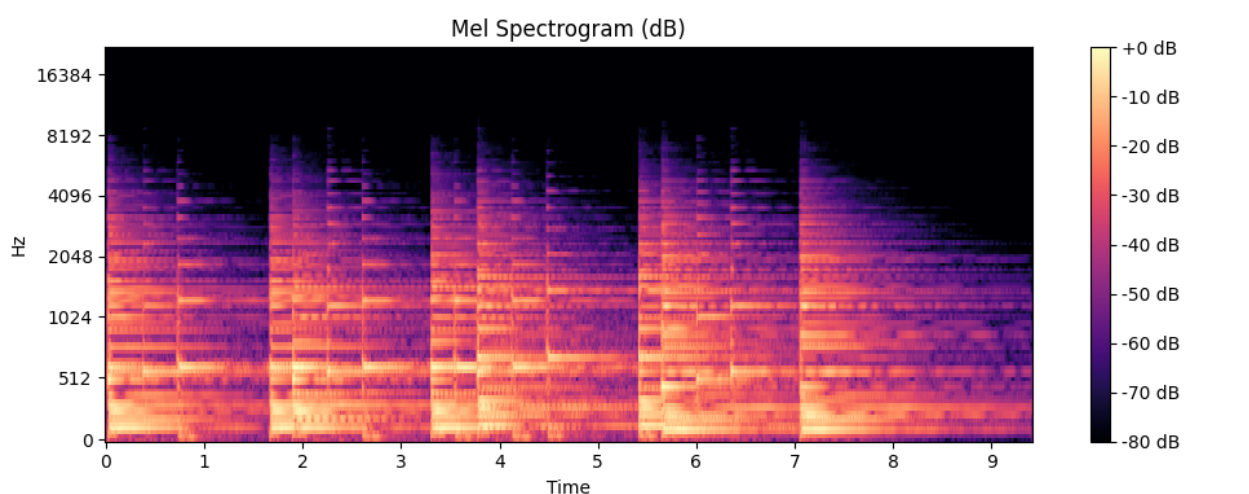
\includegraphics[width=0.8\textwidth]{钢琴.png} % 插入图片,调整宽度为页面宽度的80%
		\caption{钢琴频谱图} % 添加图片标题
	\end{figure}
	\FloatBarrier
		\href{run:小提琴.mp3}{小提琴音频}
	\begin{figure}[h]
		\centering
		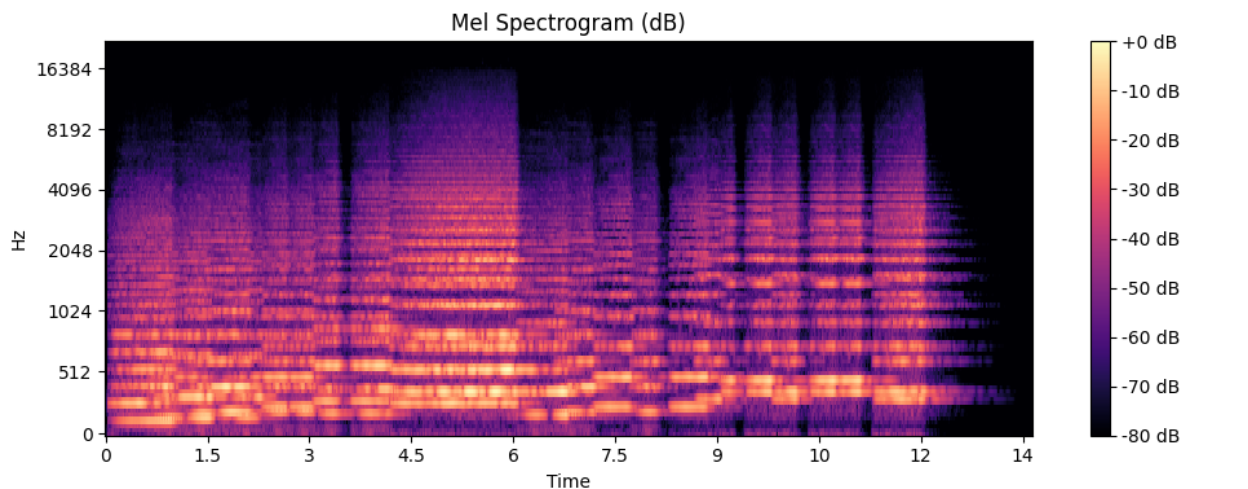
\includegraphics[width=0.8\textwidth]{小提琴.png} % 插入图片,调整宽度为页面宽度的80%
		\caption{小提琴频谱图} % 添加图片标题
	\end{figure}
	\FloatBarrier
		\href{run:长笛.mp3}{长笛音频}
	\begin{figure}[h]
		\centering
		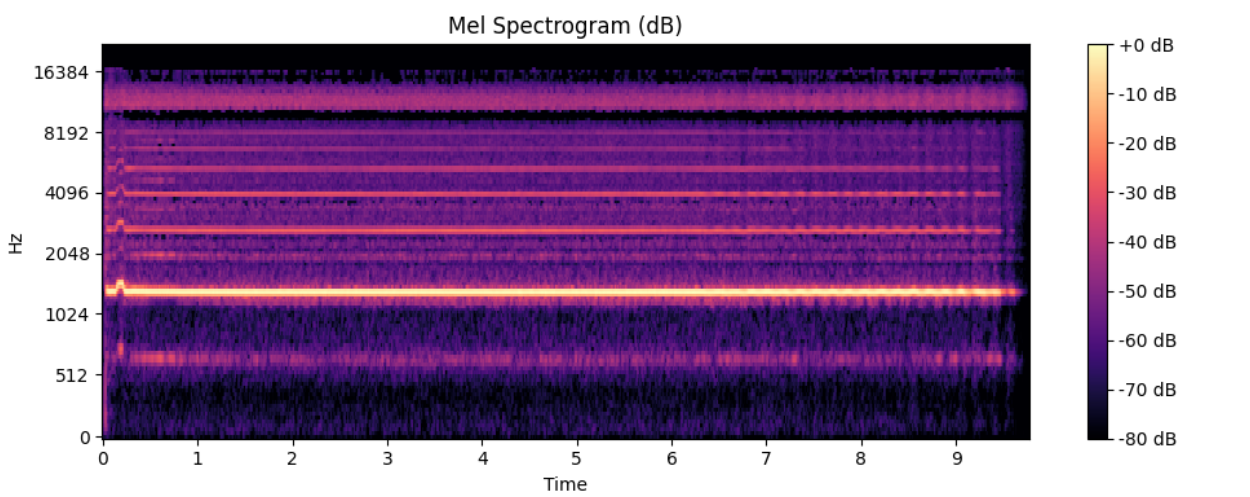
\includegraphics[width=0.8\textwidth]{长笛.png} % 插入图片,调整宽度为页面宽度的80%
		\caption{长笛频谱图} % 添加图片标题
	\end{figure}
	\FloatBarrier
	可以看出钢琴与长笛的谐波排列整齐,衰减速率不同。小提琴则具有更丰富的高频谐波与噪声成分。钢琴具有明显的瞬态攻击和衰减;长笛包络更平滑等特征。利用不同乐器间音色的区别,可以将音频中不同乐器的声音进行分离。但是要人工划定一个区分标准其实是有很大难度的,因此现在应用较广的方法是利用训练好的神经网络模型来分离声音,例如Deezer开源的音乐源分离库Spleeter提供预训练的 2、4、5 stems 模型,其中 5 stems 模型可以提取 vocals、drums、bass、piano 与 other 几个音轨,可以实现有效分离。
	\begin{thebibliography}{9}
		\bibitem{ref1}北京大学2024-2025年第二学期《数学物理方法(上)》第九次作业.
		\bibitem{ref2}\url{https://zh.wikipedia.org/wiki/\%E5\%BF\%AB\%E9\%80\%9F\%E5\%82\%82\%E9\%87\%8C\%E5\%8F\%B6\%E5\%8F\%98\%E6\%8D\%A2}
		\bibitem{ref3}\url{https://github.com/deezer/spleeter}
		\bibitem{ref4}\url{https://numpy.org/doc/stable/reference/routines.fft.html}
		\bibitem{ref5}\url{https://www.zhihu.com/question/618071093/answer/3309562922}
	\end{thebibliography}
\end{document}